\chapter{TBD}\label{ch:undefined}
En este capítulo desarrollamos el marco de trabajo realizado, las decisiones tomadas en la selección de determinados métodos expuesto en el capítulo anterior, las  herramientas utilizadas y el tipo de arquitectura seleccionada para la extracción de los datos.

\section{Pipeline}\label{sec: pipeline}
En \ac{ml} un \textit{pipeline} es el flujo de trabajo en el cual se desarrollaran las tareas, esto nos permite automatizar los datos y el flujo de tareas. Un pipeline consiste en diversos pasos donde cada uno de ellos implica determinada tarea como se menciono previamente, estos pipeline son generalmente iterativos.
%https://hackernoon.com/machine-learning-model-pipelines-part-i-e138b7a7c1ef
La construcción de pipelines proporciona muchas ventaja al igual que un desarrollo de software tradicional. Estas ventajas incluyen:
\begin{itemize}
\item \textbf{Flexibilidad}: Cada unidad, tareas, son fáciles de reemplazar de modo que si se quiere cambiar la implementación de determinada tarea se lo puede realizar sin afectar el resto del sistema.

\item \textbf{Extensibilidad}: A partir de que el sistema esta dividido se puede extender nuevas unidades, es decir, agregar nuevos pasos al flujo de trabajo de manera transparente sin afectar el correcto funcionamiento del flujo de trabajo.

\item \textbf{Legibilidad}: Al ser cada tarea atómica nos permite lograr una mejor compresión de cada una de las unidades/pasos que se desarrollaron ayudando a identificar posibles errores.

\end{itemize}

En la siguiente imagen\ref{Fig:pipeline} podemos ver un pipeline de desarrollo en aprendizaje supervisado:

\begin{figure}[H] \centering
  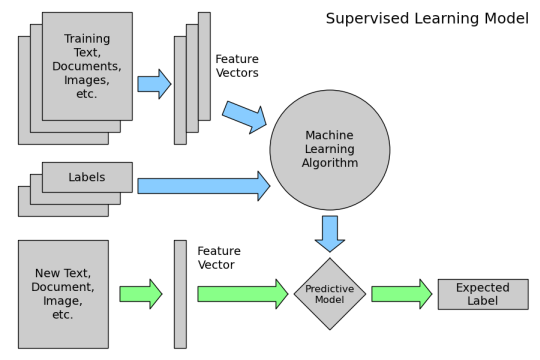
\includegraphics[height=8cm,keepaspectratio=true,clip=true]{imagenes/tbd/pipeline-sp.png}
  \caption{Pipeline}\label{Fig:pipeline}
\end{figure}

Partiendo de la figura anterior, se adapto el pipeline de acuerdo a las necesidades del trabajo de la siguiente manera:

\begin{figure}[H] \centering
  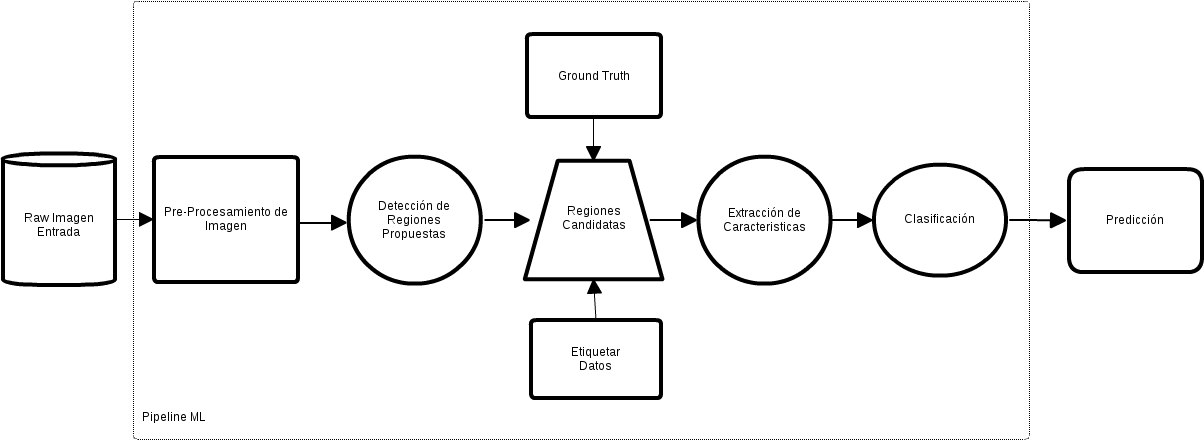
\includegraphics[height=5cm,keepaspectratio=true,clip=true]{imagenes/tbd/pipeline.png}
  \caption{Pipeline de Trabajo}\label{Fig:pipeline-mio}
\end{figure}

%https://www.datanami.com/2018/09/05/how-to-build-a-better-machine-learning-pipeline/
\subsection{Descripción del Pipeline desarrollado}\label{sub:desc-pipeline}
Descripción de cada bloque del pipeline

\subsubsection*{Pre-procesamiento}

\subsubsection*{Detección de regiones propuesta}
\subsubsection*{Regiones candidatas}
\subsubsection*{Extracción de características}
\subsubsection*{Clasificación}
\subsubsection*{Predicción}

